\chapter{Validation}\label{ch:validation}
In this section we will talk about the testing part of the project. In particular our purpose was to 
show that the system satisfy the requirements listed in ~\ref{ch:analysis}. \\
\noindent

At first, in order to do that, we wrote some test that consider different case for each state of the car:
\begin{itemize}
    \item [a.] on each side, and on the bridge itself, there aren't any cars, except the one we are testing;
    \item [b.] on the same side of our car there is another one in position -1 or 1 depending on the side, 
    while on the other one there is nobody;
    \item [c.] on the opposite side of our testing car there is another.
\end{itemize}

At a second time we decided to implement several scenarios in order to see what will actually happen. 
In the following sections there are also some significant screenshot we took from the UI while running 
different scenarios.

\subsection{Tests}
\noindent

Our tests check the correct flow of events. In other words we wanted to find out if the car in a 
particular situation (defined by the environment) reacts to it sending and receiving the expected
events. The car should also act as we wanted so that there is no accident, deadlock, starvation and so on.

\section{Functional requirements}

We were able to check if the system can:
\begin{itemize}
    \item \textbf{Coordinate the traffic}.
    \item \textbf{Avoid} any kind of \textbf{accident}.
    \item Avoid situation where more than $n$ cars, where $n$ is the capacity, cross the the bridge at 
    the same time.
    \item Make cars cars interchange messages due to decide correctly who can cross, after reached an
    (\textbf{agreement}), the bridge.
    \item Detect \textbf{broken} cars and remove them calling a tow truck.
    \item generate new cars.
\end{itemize}


\section{Non functional requirements}

For the non functional requirements we tested that:
\begin{itemize}
    \item \textbf{Safety}: the system guarantees that the bridge can be crossed only by cars that 
        are moving in the same direction, but also that if a car broke, the others are able to detect that
        and so they stop before crashing into it. 
    \item \textbf{Strength}: the system is usable even if a car breaks down and needs to be removed.
    \item \textbf{Scalability}: incrementing number of cars, clients and web services, the system don't affect
    too much the whole system.
    \item \textbf{Starvation}: when a car requires to cross the bridge, the request will be satisfied 
    eventually. 
    \item \textbf{Fairness}: the crossing order is a \textbf{FIFO ordering}.
\end{itemize}

In order to detacht any type of failure we defined different $scenarios$: these are json files which instantiate
different number and type of cars. The following are the property of each scenario:
\begin{itemize}
    \item[scenario \textbf{1}]: \\ there are two cars, on the same side (left), while there is no one on the other 
    side. The cars don't arrive at the same time but there is a delay of 2000ms between them. \\
    The correct behaviour should be that the first car that reach the bridge will cross it (the other 
    one will wait and then cross the bridge too) \\
    \begin{center}
        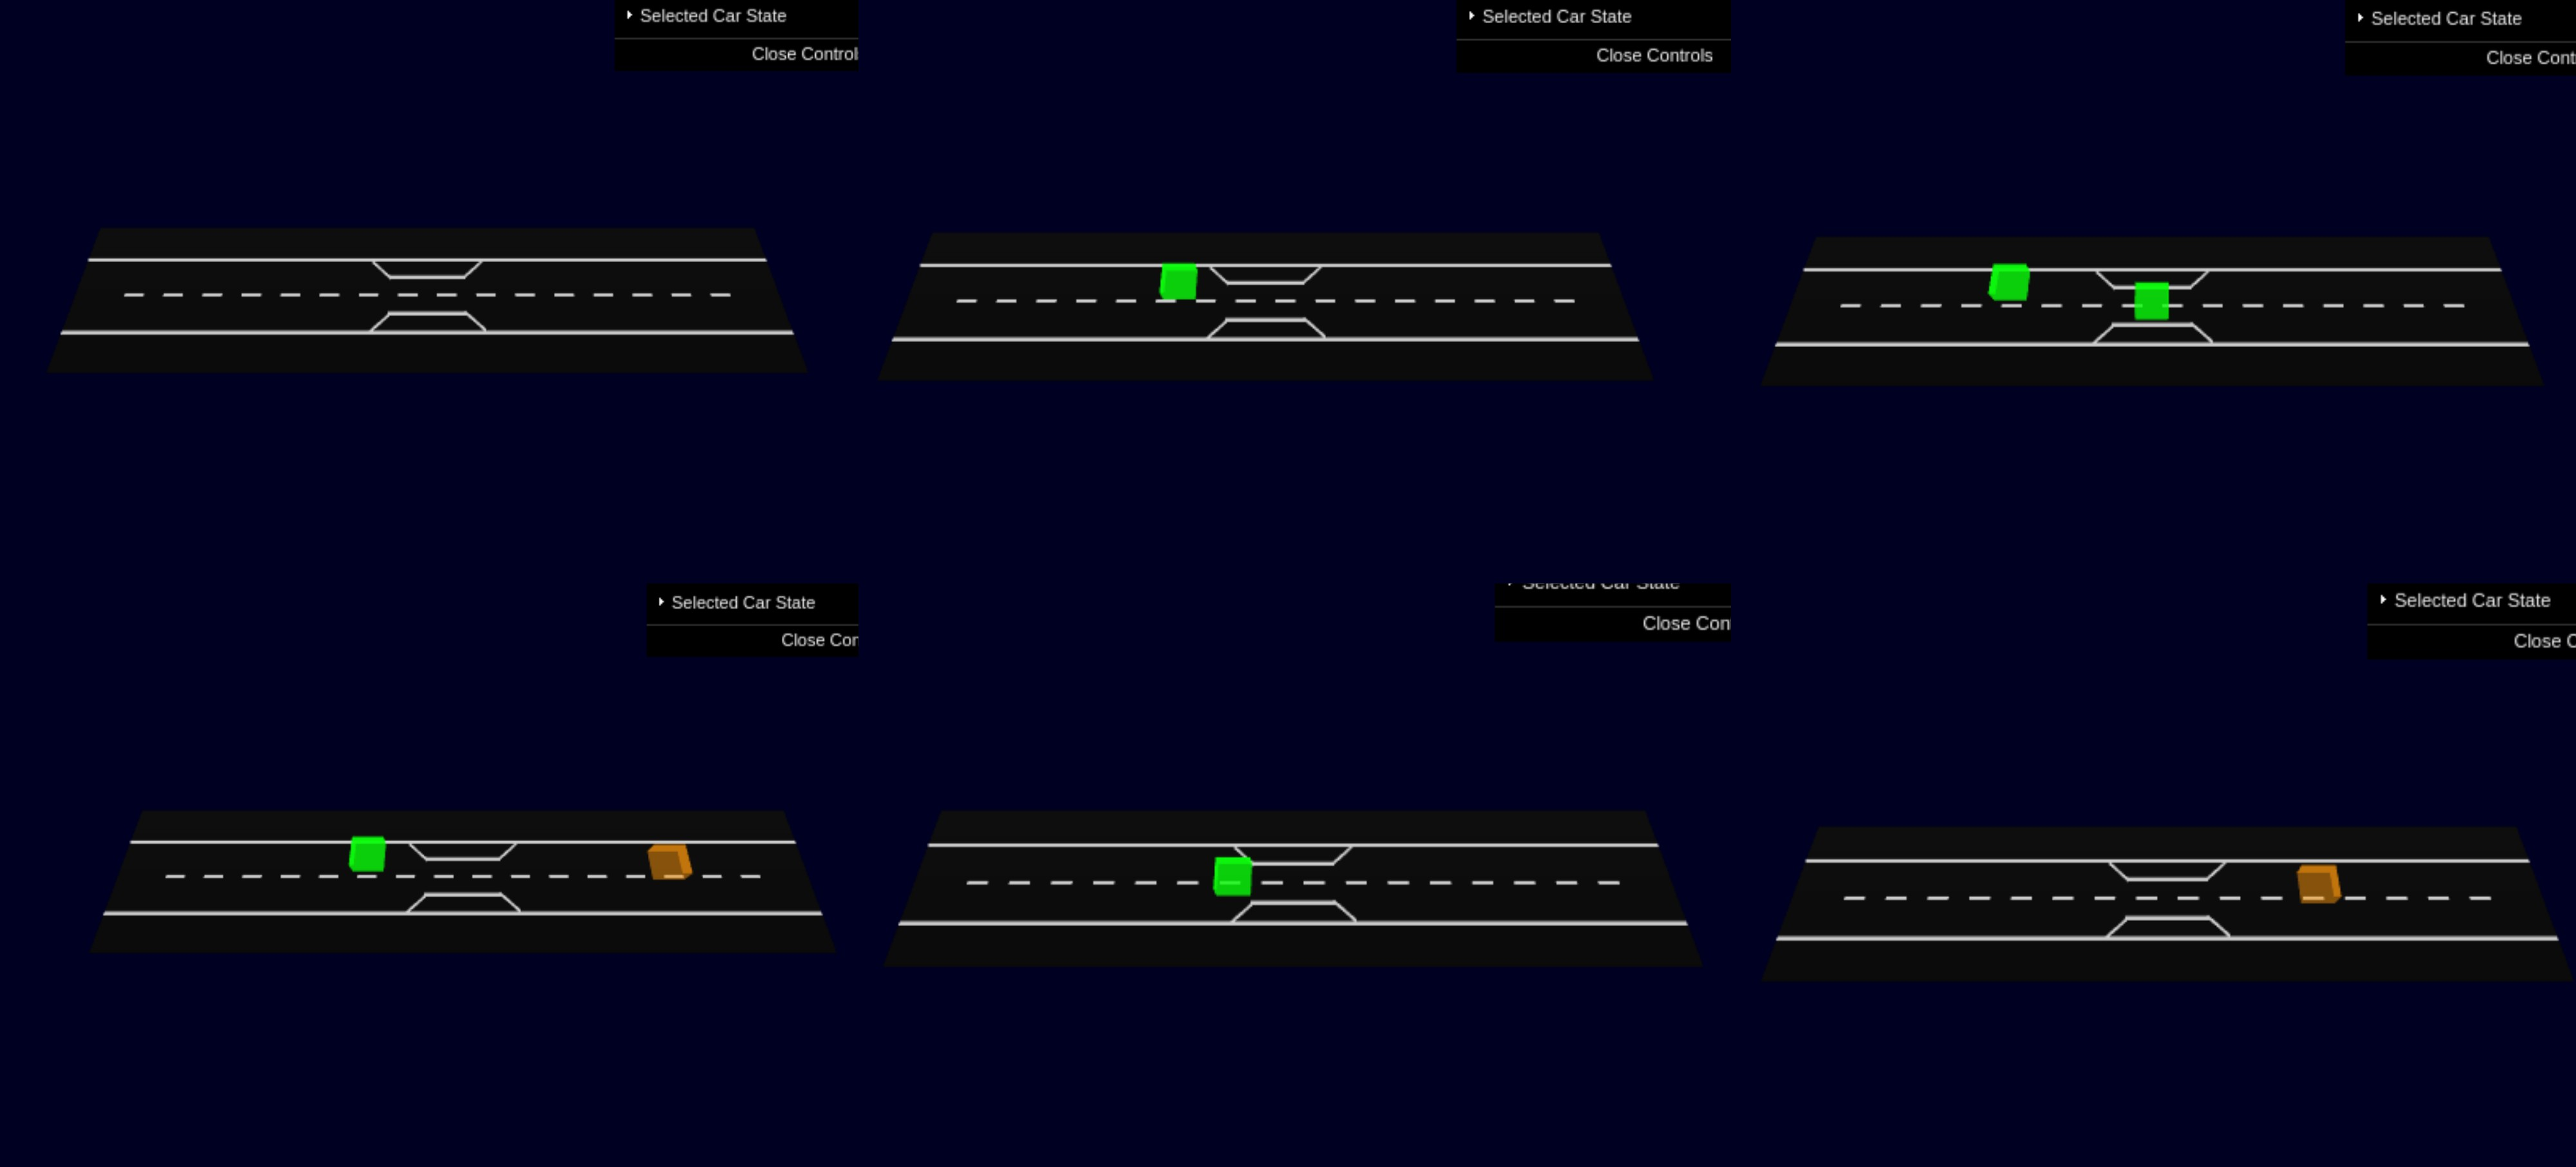
\includegraphics[scale=0.3, width=\linewidth]{assets/sc1.jpg}
        \captionof{figure}{Scenario 1}
    \end{center}
    \item[scenario \textbf{2}]: \\ there are four car from the same side all created at the same time \\The correct behaviour should be that 
    the cars are able to synchronize themselves and then cross the bridge according to their $arrival\_time$
    \\
    \begin{center}
        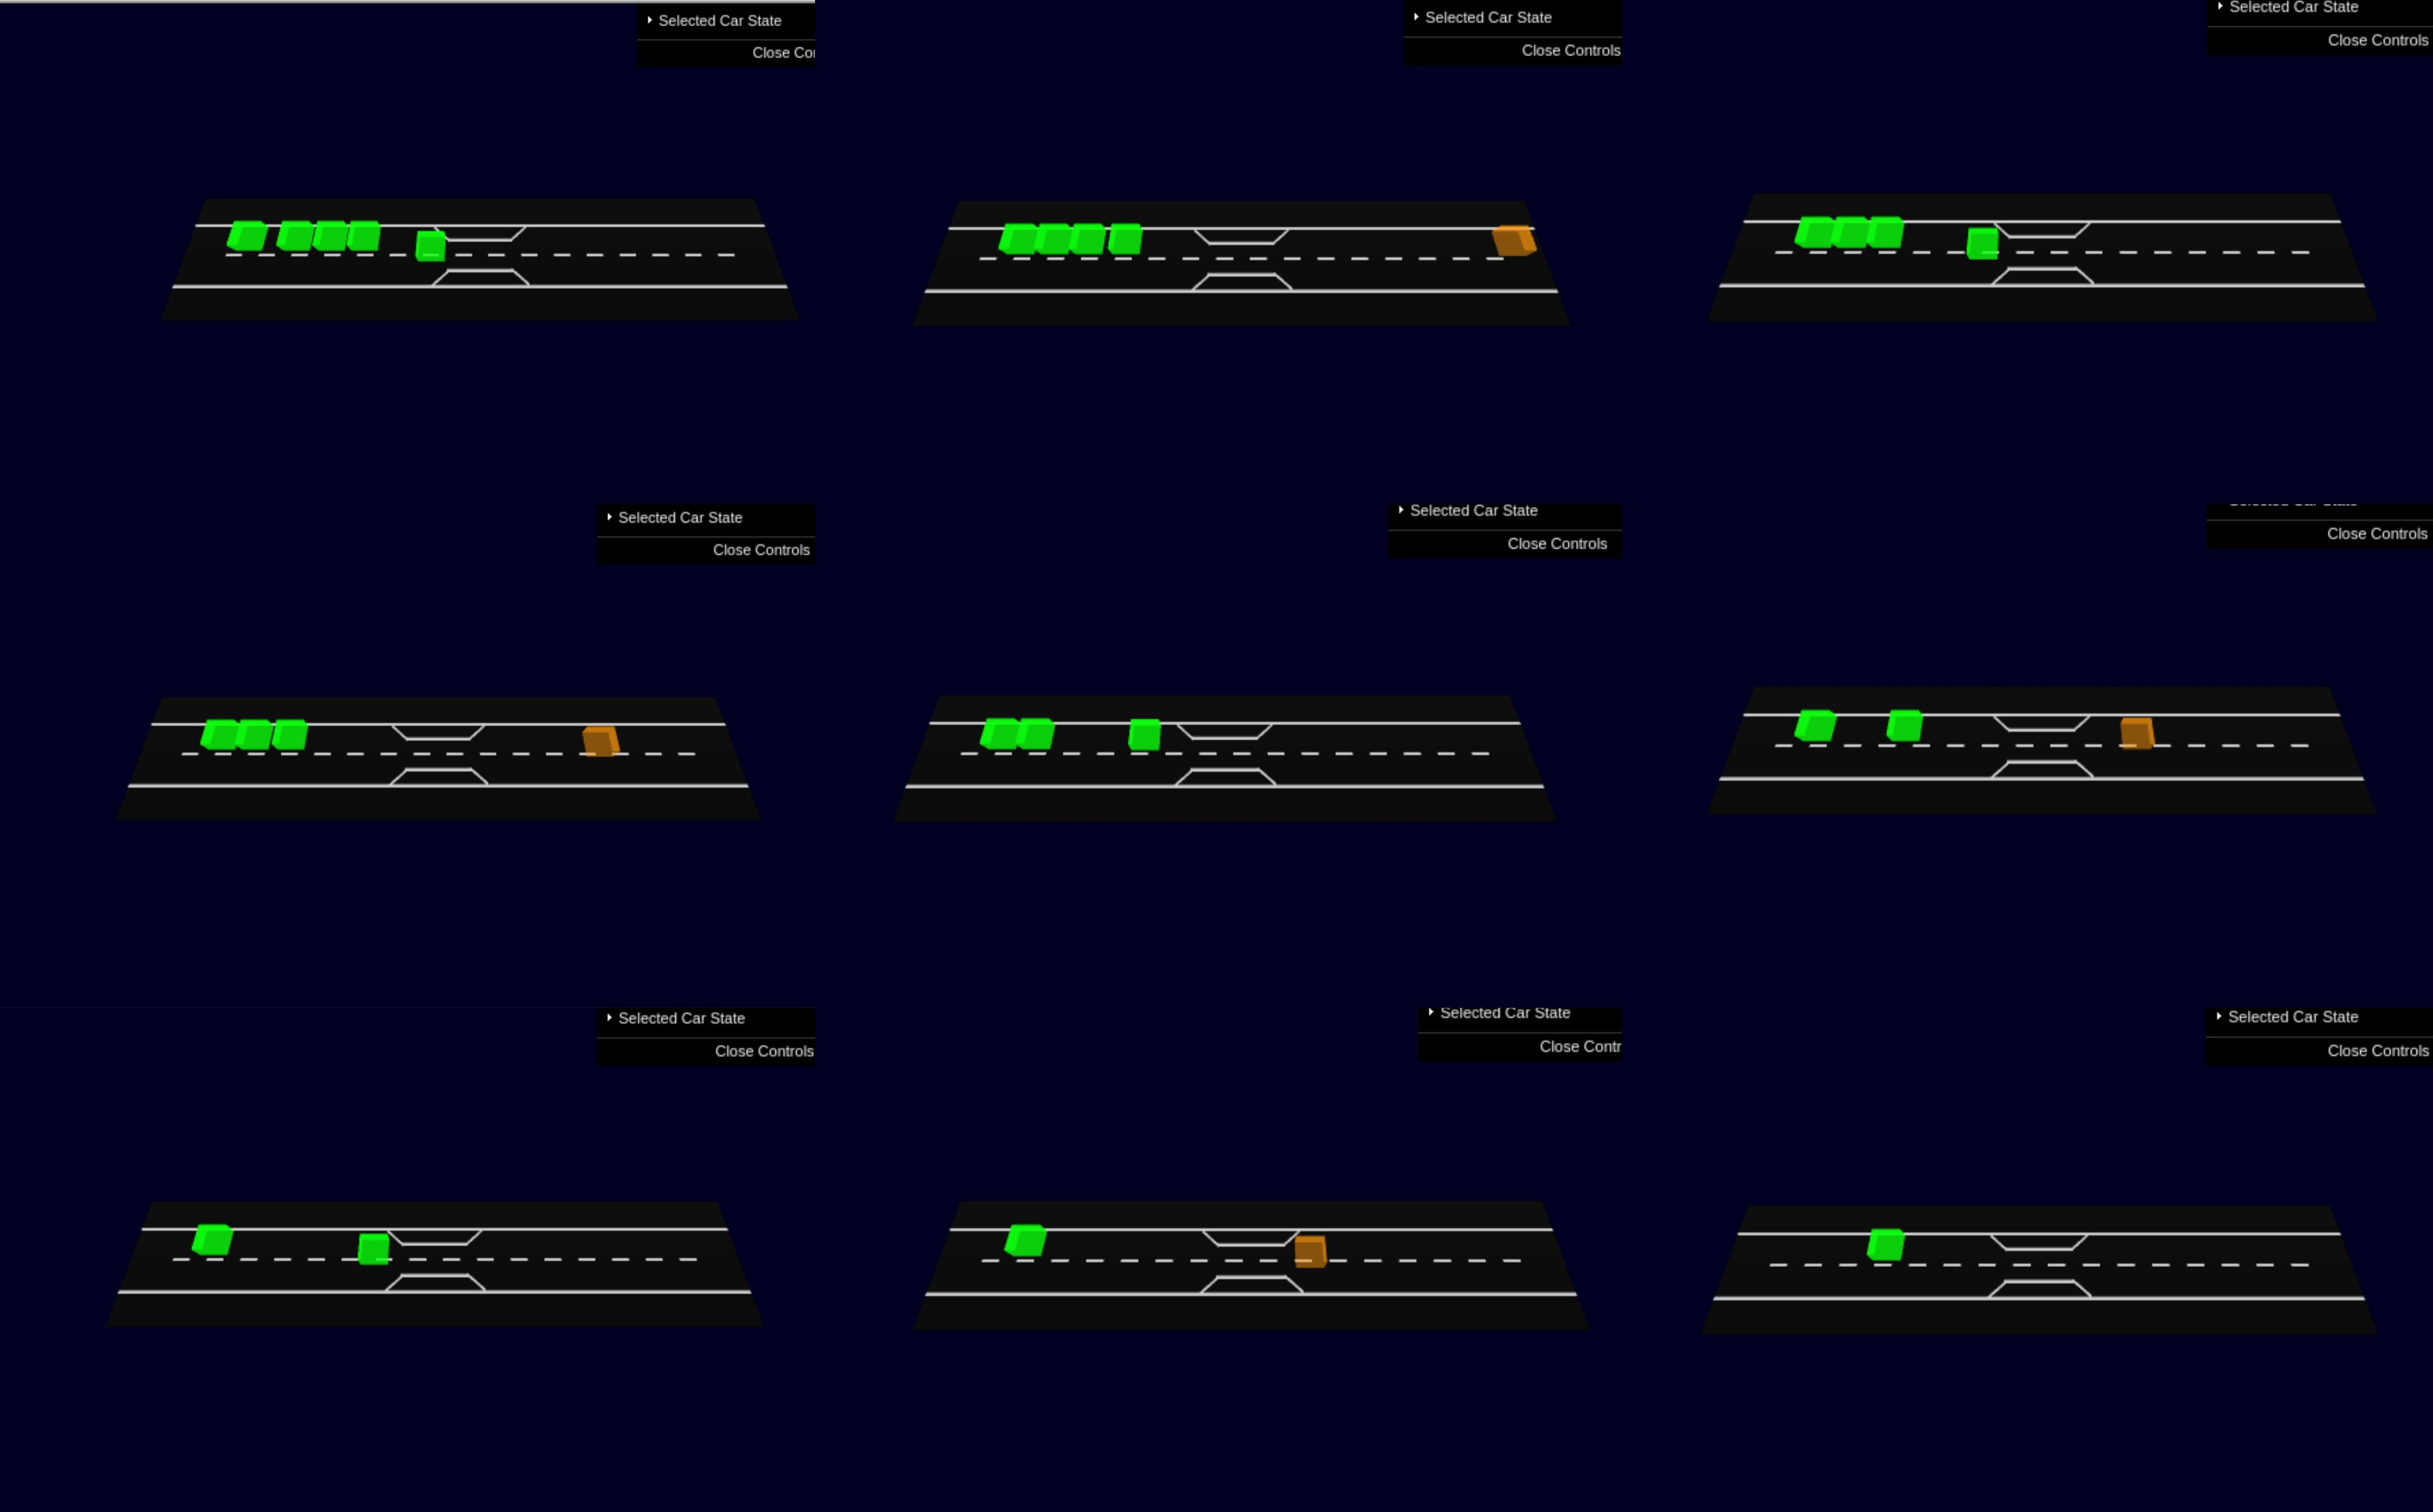
\includegraphics[scale=0.3, width=\linewidth]{assets/sc2.jpg}
        \captionof{figure}{Scenario 2}
    \end{center}
    \item[scenario \textbf{3}]: \\ there are four car on left side and one on the right side (there is no delay 
    between them).\\ The correct behaviour should be that the cars will cross the bridge in the correct 
    order without crashing with the car on the other side (that will wait for its turn accordingly
    to its arrival time) \\
    \begin{center}
        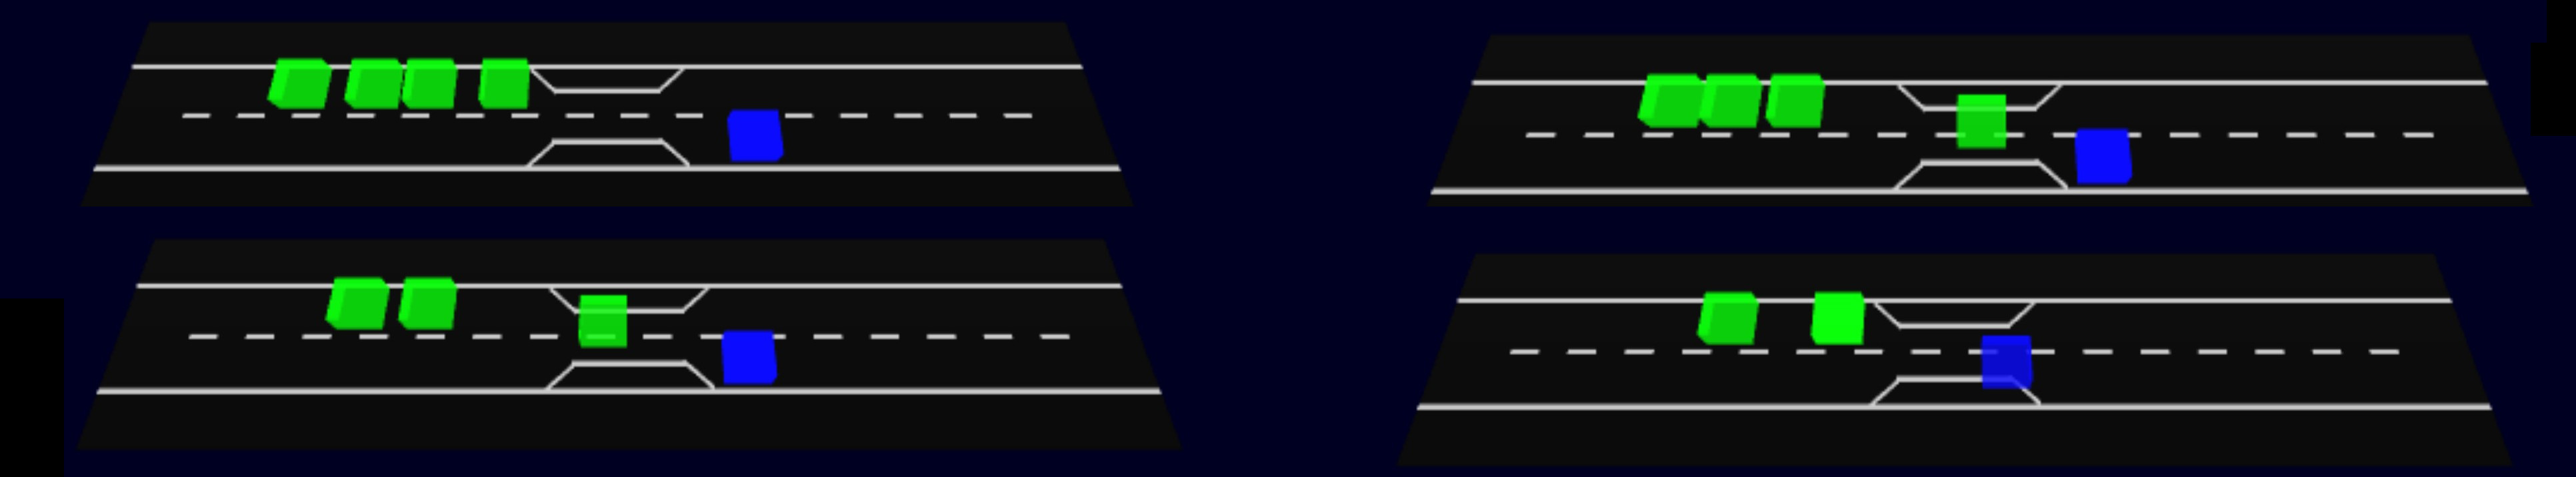
\includegraphics[scale=0.3, width=\linewidth]{assets/sc3.jpg}
        \captionof{figure}{Scenario 3}
    \end{center}
    \item[scenario \textbf{4}]: \\ there are three cars, with no delay, that are on the same side but there is one that is going to
    have a system crash.\\ The correct behaviour should be that the two cars that won't have any type of crash
    will cross the bridge even if there is one in front of them that has crashed. Due to the fact that the 
    $crash\_type$ for the broken one is 2, the other cars (at least one of them) have to call the tow truck for 
    it; after it has been removed the cars can continue crossing the bridge
    \item[scenario \textbf{5}]: \\ there are five cars that are on the same side and all of them have a crash; three of them have system crash, 
    while the other have only engine crash and there is a delay between the car with $crash\_type$ 2 and the others.\\
    The correct behaviour should be that the cars that have only engine crash will call the tow truck for themselves and
    for the cars that they can reach (because if a car has system crash cannot call a tow truck for itself). 
    For this reason if there is a car that has a system crash after that the cars, which had an engine crash, 
    have already been removed by the tow truck, it will stuck there, waiting for a new car to call the tow truck for it
    \item[scenario \textbf{6}]: \\ there are two cars that will have a crash with $crash\_type$ 2 and another one that will not
    crash and that will arrive after that the previously cars have crashed due to the delay between them. All of them are on the same 
    side of the bridge. \\ The correct behaviour should be that the cars with 
    the crash will wait there until the other one arrive and call a tow truck for them. After they have been removed
    the last car can cross the bridge 
    \item[scenario \textbf{7}]: \\ it is the same as the above but there are only two cars and them are on different sides; the 
    sane one has a delay. \\ The correct behaviour should be that when it arrives, it will call the tow truck for
    the other and then cross the bridge (after the other has been removed) 
    \item[scenario \textbf{8}]: \\ there are five cars on the same side but only one (with the longer delay) is sane. \\
    The correct behaviour should be that the cars with crashes will wait to be removed by the tow truck called 
    by the sane one (they have $crash\_type$ 2) and then the last car can cross the bridge 
    \item[scenario \textbf{9}]: \\ the first three cars that arrive are two on the left side and one of them will
    have a system crash, while the other one is on the right side. After a delay of 300ms other 10 cars (four from one side, and six from the other)
    will arrive and they will not have any type of crash. \\
    The correct behaviour should be that the cars with crashes will wait to be removed by the tow truck called by
    the one of the first three that is sane or by the others that will arrive after.    
    \item[scenario \textbf{10}]: \\ there are three cars, two from the same side. One of them has a system crash 
    and a delay of 300ms. \\
    The correct behaviour should be that the car with crash will wait to be removed by the tow truck called by
    one or both the others cars.
    
    
\end{itemize}